% Fuente: Pauta del Auxiliar 8, «Métodos de programación entera».
\begin{enumerate}
  \item[(a)] Gráficando el conjunto factible se tiene:
  \begin{figure}
      \centering
      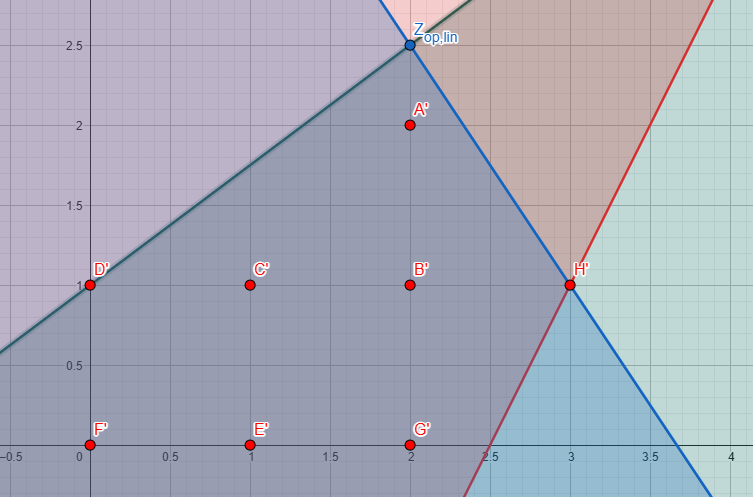
\includegraphics[width=0.7\linewidth]{img/ejercicios/Capitulo-5/ejercicio_5_2_metodos_programacion_entera.png}
      \caption{Conjunto factible Pregunta 3.}
      \label{ex:5:2:fig:conjunto-factible}
  \end{figure}
  La solución de la relajación lineal y del problema original son:
  \[
    z_{\text{LP}} = 7,\quad\text{en }(x_{1},x_{2})=(2,2.5),
    \qquad
    z_{\text{IP}} = 6,\quad\text{en }(x_{1},x_{2})=(2,2).
  \]
  
  \item[(b)] Si se enumeran las soluciones enteras factibles:
  \[
  \{(0,0),(1,0),(2,0),(0,1),(1,1),(2,1),(2,2),(3,1)\}
  \]
  su envoltura convexa es el polígono de vértices
  \[
    \{(0,0),\quad(2,0),\quad(3,1),\quad(2,2),\quad(0,1).\}
  \]
  Es decir,
  \[
    \mathrm{conv}\bigl\{(0,0),(2,0),(3,1),(2,2),(0,1)\bigr\}.
  \]
  Las siguientes rectas producen la envoltura convexa:
  \begin{align*}
      & x_1\geq0\\
      & x_2 \geq 0\\
      & x_2 \geq x_1 -2 \\
      & x_2 \leq 0.5 x_1 +1\\
      & x_2 \leq -x_1 +4
  \end{align*}
  
  \item[(c)] Las matrices del problema relajado en formulación estándar son:
  \[
  A=\begin{pmatrix}
    -3 & 4 &1 & 0 & 0 \\
    3 & 2 & 0 &1&0 \\
    2 & -1&0&0&1
\end{pmatrix}, \quad b= \begin{pmatrix}
    4 \\
    11 \\
    5 
\end{pmatrix}, \quad B=
    \begin{pmatrix}
        -3 & 4 &0  \\
        3 & 2 & 0  \\
        2 & -1&1
    \end{pmatrix}
  \]
  El óptimo de la relajación lineal es $(2,2.5,0,0,5.3)$, luego se realiza el corte sobre $x_2$:
  \begin{equation}
      x_2 + \lfloor\overline{a_{23}}\rfloor \cdot s_1+\lfloor\overline{a_{24}}\rfloor \cdot s_2 \leq \lfloor\overline{a_{20}}\rfloor
  \end{equation}
  donde:
  \begin{align}
     & \overline{a_{23}}=\left(B^{-1}\begin{pmatrix}
          1  \\ 0 \\ 0
      \end{pmatrix} \right)_2 =\frac{1}{6} \\
    & \overline{a_{23}}=\left(B^{-1}\begin{pmatrix}
          0  \\ 1 \\ 0
    \end{pmatrix} \right)_2 =\frac{1}{6} \\
    & \overline{a_{23}}=\left(B^{-1}b \right)_2 =2.5
  \end{align}
De modo que el nuevo corte es:
\begin{equation}
    x_2 \leq 2
\end{equation}
  
  \item[(d)] Comenzamos con $L=-\infty$, donde L corresponde a la mejor corta inferior al ser un problema de maximización.
  
  El nodo raíz corresponde a resolver la relajación lineal del problema original, luego $(x_1, x_2)=(2,2.5)$, donde $z=7$. Dado que no tiene solución entera, se selecciona $x_2$ para particionar el conjunto factible. No se actualiza la cota ($L=-\infty$).

  Los subproblemas generados son:

\begin{equation}
\begin{aligned}
(P2)\quad \min\;& -x_1 \;-\; 2x_2 \\
\text{s.a.}\;& -3x_{1} + 4x_{2} \le 4,\\
& 3x_{1} + 2x_{2} \le 11,\\
& 2x_{1} - x_{2} \le 5,\\
& x_{2} \le 2,\\
& x_{i} \ge 0,\quad i\in\{1,2\}.
\end{aligned}
\end{equation}

\begin{equation}
\begin{aligned}
(P3)\quad \min\;& -x_1 \;-\; 2x_2 \\
\text{s.a.}\;& -3x_{1} + 4x_{2} \le 4,\\
& 3x_{1} + 2x_{2} \le 11,\\
& 2x_{1} - x_{2} \le 5,\\
& x_{2} \ge 3,\\
& x_{i} \ge 0,\quad i\in\{1,2\}.
\end{aligned}
\end{equation}

Dado que el problema $(P3)$ es infactible, se descarta. El problema $(P2)$ alcanza el óptimo en:
\begin{equation}
    x=\left(\frac{7}{3},2\right), \quad z= \frac{19}{3}
\end{equation}
    
Como la solución es no entera, se elige $x_1$ para particionar el conjunto. Aún no hay solución entera, por lo que $L=-\infty$.

Los subproblemas generados a partir de $(P2)$ son:

\begin{equation}
\begin{aligned}
(P4)\quad \min\;& -x_1 \;-\; 2x_2\\
\text{s.a.}\;& -3x_{1} + 4x_{2} \le 4,\\
& 3x_{1} + 2x_{2} \le 11,\\
& 2x_{1} - x_{2} \le 5,\\
& x_{2} \le 2,\\
& x_{1} \le 2,\\
& x_{i} \ge 0,\quad i\in\{1,2\}.
\end{aligned}
\end{equation}

\begin{equation*}
\begin{aligned}
(P5)\quad \min\;& -x_1 \;-\; 2x_2\\
\text{s.a.}\;& -3x_{1} + 4x_{2} \le 4,\\
& 3x_{1} + 2x_{2} \le 11,\\
& 2x_{1} - x_{2} \le 5,\\
& x_{2} \le 2,\\
& x_{1} \ge 3,\\
& x_{i} \ge 0,\quad i\in\{1,2\}.
\end{aligned}
\end{equation*}

La solución de $(P4)$ es:
\begin{equation}
    x=(2,2), \quad z=6
\end{equation}
 Como la solución es entera, se actualiza la cota $L=6$.

 La solución de $(P5)$ es:
 \begin{equation}
     x=(3,1), \quad z= 5
 \end{equation}
 Dado que $z\le L$, se descarta $(P5)$ y la cota superior se mantiene en $L=6$.

 Finalmente, tras explorar todos los nodos, la mejor solución entera es:
 \begin{equation}
    x=(2,2), \quad z=6
\end{equation}
la cual corresponde a la solución del problema original.
  
  \item[(e)] Dado que se está maximizando, se obtendrán cotas superiores. Al relajar dicha restricción con multiplicador \(p\ge0\), el lagrangiano queda:
    \[
      Z(p)
      = \max_{x_{1},x_{2}}
      \Bigl\{\,x_{1} + 2x_{2}
      \;+\; p\,(4 + 3x_{1} - 4x_{2})\Bigr\}
      \quad\text{s.a.}\quad
      \begin{cases}
        3\,x_{1} + 2\,x_{2} \;\le\; 11,\\
        2\,x_{1} - x_{2} \;\le\; 5,\\
        x_{1},x_{2}\ge0,\;x_{1},x_{2}\in\mathbb{Z}.
      \end{cases}
    \]
    Los puntos factibles \((x_{1},x_{2})\) (ignorando la restricción dualizada) generan las siguientes funciones candidatas
    \(\displaystyle\overline{Z}(p)=x_{1}+2x_{2}+p\,(4+3x_{1}-4x_{2})\):

    \[
      \begin{array}{cc|c}
        \hline
        x_{1} & x_{2} & \overline{Z}(p) \\ \hline
        0 & 0 & 4\,p              \\
        0 & 1 & 2                  \\
        0 & 2 & 4 - 4\,p          \\
        0 & 3 & 6 - 8\,p          \\
        0 & 4 & 8 -12\,p          \\
        0 & 5 & 10-16\,p          \\[4pt]
        1 & 0 & 1 + 7\,p          \\
        1 & 1 & 3 + 3\,p          \\
        1 & 2 & 5 -   p          \\
        1 & 3 & 7 - 5\,p          \\
        1 & 4 & 9 - 9\,p          \\[4pt]
        2 & 0 & 2 +10\,p          \\
        2 & 1 & 4 + 6\,p          \\
        2 & 2 & 6 + 2\,p          \\[4pt]
        3 & 1 & 5 + 9\,p          \\
        \hline
      \end{array}
    \]

    A partir de aquí se toma el envolvente superior de estas rectas para obtener
    \(\;Z(p)=\max_{i,j}\overline{Z}(p)\;\) y luego
    \(\displaystyle Z_{D}=\min_{p\ge0}Z(p)\).

Tomando las funciones candidatas \(\overline{Z}(p)=x_{1}+2x_{2}+p(4+3x_{1}-4x_{2})\)
    en cada punto factible y construyendo el envolvente superior, resulta:
    \[
      Z(p)
      = \max_{(i,j)}\overline{Z}(p)
      = 
      \begin{cases}
        10 - 16\,p, & 0 \le p \le \tfrac17,\\[0.3em]
        9 - 9\,p,   & \tfrac17 \le p \le \tfrac29,\\[0.3em]
        5 + 9\,p,   & \tfrac29 \le p \le 3,\\[0.3em]
        2 +10\,p,   & p \ge 3.
      \end{cases}
    \]
    La mejor cota dual se halla en la intersección de la recta $9+9p$ y $5+9p$:
    \[
      \min_{p\ge0}Z(p)
      \;\Longrightarrow\;
      p^* = \tfrac29,
      \quad Z_{D} = Z\bigl(\tfrac29\bigr) = 7.
    \]

Ahora, al relajar la restricción
    \[
      2x_{1} - x_{2} \le 5
    \]
    con lagrangiano
    \[
      Z(q)
      = \max_{x_{1},x_{2}}
      \Bigl\{\,x_{1} + 2x_{2}
      \;+\; q\,(5 - 2x_{1} + x_{2})\Bigr\}
      \quad\text{s.a.}\quad
      \begin{cases}
        -3x_{1} + 4x_{2} \;\le\; 4,\\
        3x_{1} + 2x_{2} \;\le\; 11,\\
        x_{1},x_{2}\ge0,\;x_{1},x_{2}\in\mathbb{Z}.
      \end{cases}
    \]

    Los puntos factibles \((x_{1},x_{2})\) (ignorando la restricción dualizada) generan las siguientes funciones candidatas:

    \[
      \begin{array}{cc|c}
      \hline
      x_{1} & x_{2} & \overline{Z}(q) \\ \hline
      0 & 0 & 0 + 5q \\
      0 & 1 &  2 + 6q \\
      1 & 0 & 1 + 3q \\
      1 & 1 & 3 + 4q \\
      2 & 0 & 2 + 1q \\
      2 & 1 & 4 + 2q \\
      2 & 2 & 6 + 3q \\
      3 & 0 & 3 - 1q \\
      3 & 1 & 5 + 0q \\ \hline
      \end{array}
    \]

    El valor dual es el envolvente superior de estas rectas:
    \[
      Z(q)
      =
      \begin{cases}
        6 + 3q, & 0 \le q \le \tfrac{4}{3},\\[0.3em]
        2 + 6q, & q \ge \tfrac{4}{3}.
      \end{cases}
    \]
    Como ambas ramas tienen pendiente positiva, el mínimo sobre \(q\ge0\) se logra en
    \[
      q^* = 0,
      \qquad
      Z_{D} = Z(0) = 6.
    \]
\end{enumerate}
